\documentclass[1p]{elsarticle_modified}
%\bibliographystyle{elsarticle-num}

%\usepackage[colorlinks]{hyperref}
%\usepackage{abbrmath_seonhwa} %\Abb, \Ascr, \Acal ,\Abf, \Afrak
\usepackage{amsfonts}
\usepackage{amssymb}
\usepackage{amsmath}
\usepackage{amsthm}
\usepackage{scalefnt}
\usepackage{amsbsy}
\usepackage{kotex}
\usepackage{caption}
\usepackage{subfig}
\usepackage{color}
\usepackage{graphicx}
\usepackage{xcolor} %% white, black, red, green, blue, cyan, magenta, yellow
\usepackage{float}
\usepackage{setspace}
\usepackage{hyperref}

\usepackage{tikz}
\usetikzlibrary{arrows}

\usepackage{multirow}
\usepackage{array} % fixed length table
\usepackage{hhline}

%%%%%%%%%%%%%%%%%%%%%
\makeatletter
\renewcommand*\env@matrix[1][\arraystretch]{%
	\edef\arraystretch{#1}%
	\hskip -\arraycolsep
	\let\@ifnextchar\new@ifnextchar
	\array{*\c@MaxMatrixCols c}}
\makeatother %https://tex.stackexchange.com/questions/14071/how-can-i-increase-the-line-spacing-in-a-matrix
%%%%%%%%%%%%%%%

\usepackage[normalem]{ulem}

\newcommand{\msout}[1]{\ifmmode\text{\sout{\ensuremath{#1}}}\else\sout{#1}\fi}
%SOURCE: \msout is \stkout macro in https://tex.stackexchange.com/questions/20609/strikeout-in-math-mode

\newcommand{\cancel}[1]{
	\ifmmode
	{\color{red}\msout{#1}}
	\else
	{\color{red}\sout{#1}}
	\fi
}

\newcommand{\add}[1]{
	{\color{blue}\uwave{#1}}
}

\newcommand{\replace}[2]{
	\ifmmode
	{\color{red}\msout{#1}}{\color{blue}\uwave{#2}}
	\else
	{\color{red}\sout{#1}}{\color{blue}\uwave{#2}}
	\fi
}

\newcommand{\Sol}{\mathcal{S}} %segment
\newcommand{\D}{D} %diagram
\newcommand{\A}{\mathcal{A}} %arc


%%%%%%%%%%%%%%%%%%%%%%%%%%%%%5 test

\def\sl{\operatorname{\textup{SL}}(2,\Cbb)}
\def\psl{\operatorname{\textup{PSL}}(2,\Cbb)}
\def\quan{\mkern 1mu \triangleright \mkern 1mu}

\theoremstyle{definition}
\newtheorem{thm}{Theorem}[section]
\newtheorem{prop}[thm]{Proposition}
\newtheorem{lem}[thm]{Lemma}
\newtheorem{ques}[thm]{Question}
\newtheorem{cor}[thm]{Corollary}
\newtheorem{defn}[thm]{Definition}
\newtheorem{exam}[thm]{Example}
\newtheorem{rmk}[thm]{Remark}
\newtheorem{alg}[thm]{Algorithm}

\newcommand{\I}{\sqrt{-1}}
\begin{document}

%\begin{frontmatter}
%
%\title{Boundary parabolic representations of knots up to 8 crossings}
%
%%% Group authors per affiliation:
%\author{Yunhi Cho} 
%\address{Department of Mathematics, University of Seoul, Seoul, Korea}
%\ead{yhcho@uos.ac.kr}
%
%
%\author{Seonhwa Kim} %\fnref{s_kim}}
%\address{Center for Geometry and Physics, Institute for Basic Science, Pohang, 37673, Korea}
%\ead{ryeona17@ibs.re.kr}
%
%\author{Hyuk Kim}
%\address{Department of Mathematical Sciences, Seoul National University, Seoul 08826, Korea}
%\ead{hyukkim@snu.ac.kr}
%
%\author{Seokbeom Yoon}
%\address{Department of Mathematical Sciences, Seoul National University, Seoul, 08826,  Korea}
%\ead{sbyoon15@snu.ac.kr}
%
%\begin{abstract}
%We find all boundary parabolic representation of knots up to 8 crossings.
%
%\end{abstract}
%\begin{keyword}
%    \MSC[2010] 57M25 
%\end{keyword}
%
%\end{frontmatter}

%\linenumbers
%\tableofcontents
%
\newcommand\colored[1]{\textcolor{white}{\rule[-0.35ex]{0.8em}{1.4ex}}\kern-0.8em\color{red} #1}%
%\newcommand\colored[1]{\textcolor{white}{ #1}\kern-2.17ex	\textcolor{white}{ #1}\kern-1.81ex	\textcolor{white}{ #1}\kern-2.15ex\color{red}#1	}

{\Large $\underline{12a_{1066}~(K12a_{1066})}$}

\setlength{\tabcolsep}{10pt}
\renewcommand{\arraystretch}{1.6}
\vspace{1cm}\begin{tabular}{m{100pt}>{\centering\arraybackslash}m{274pt}}
\multirow{5}{120pt}{
	\centering
	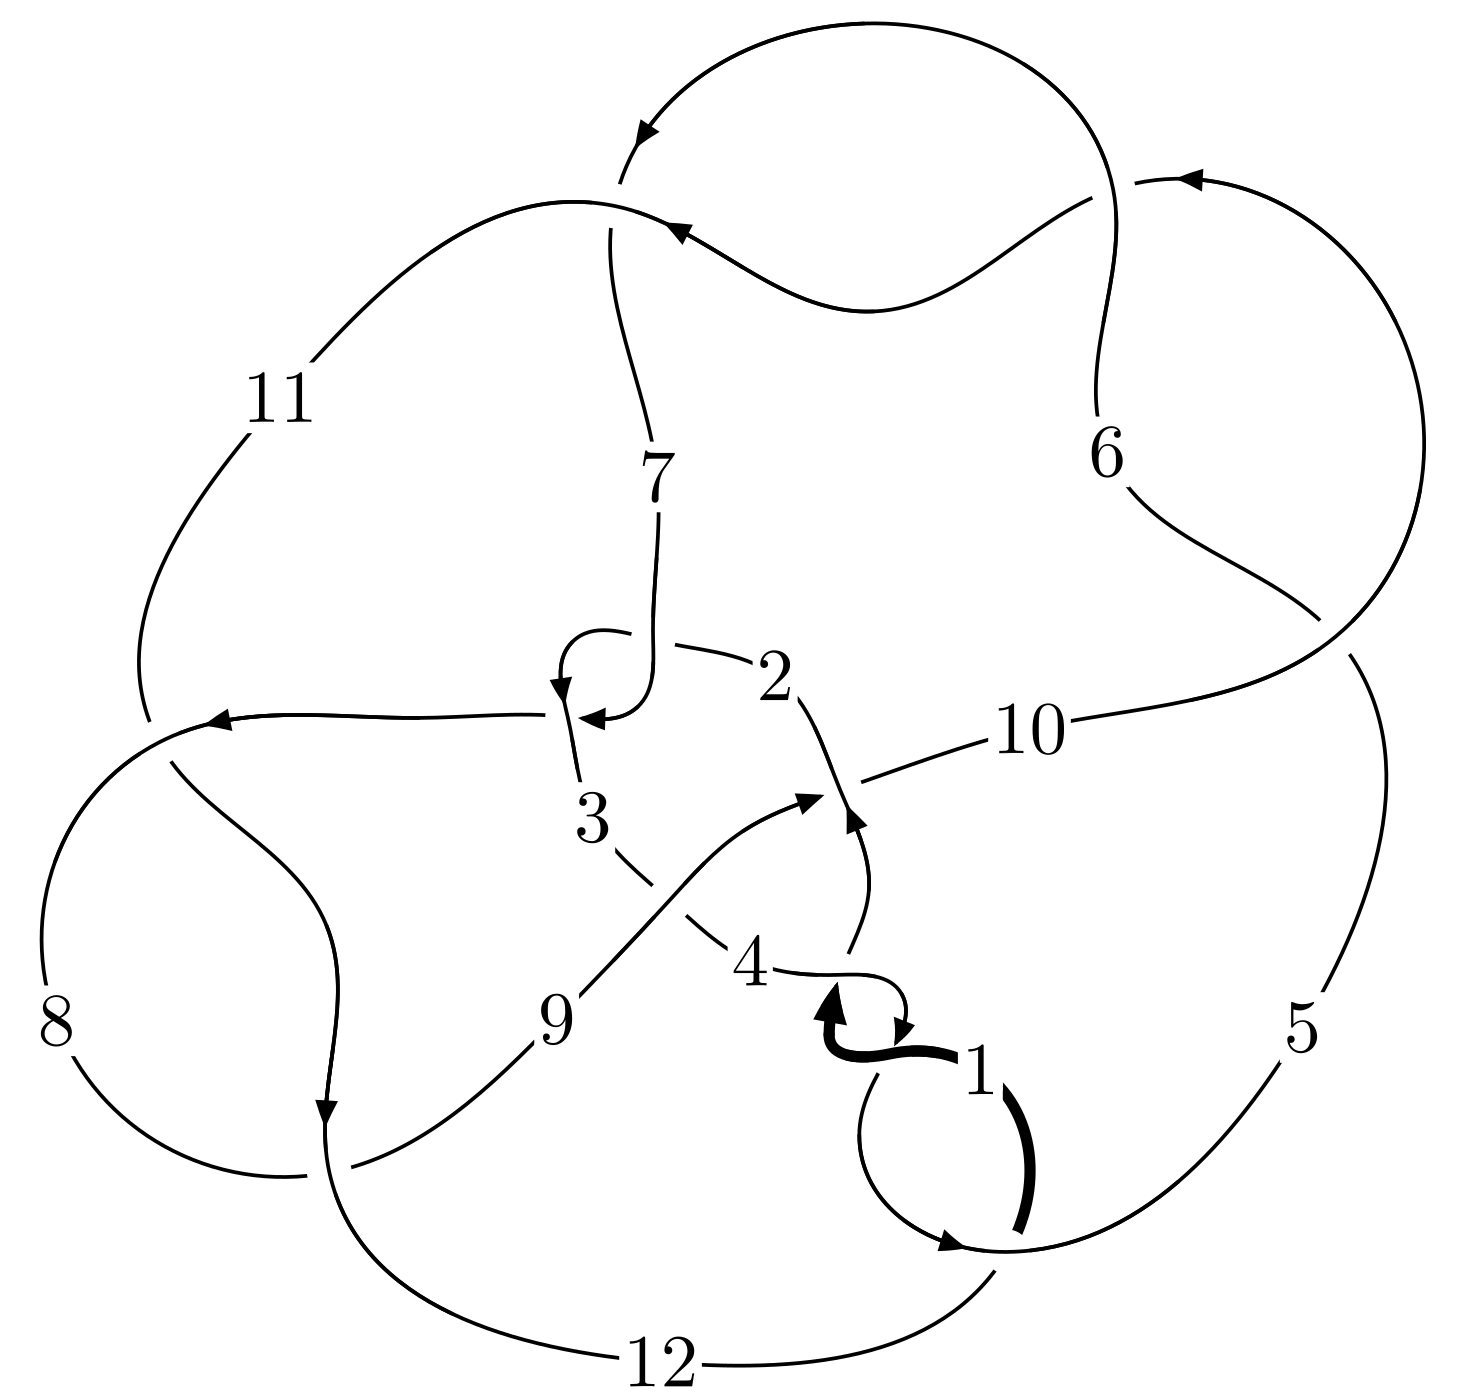
\includegraphics[width=112pt]{../../../GIT/diagram.site/Diagrams/png/1867_12a_1066.png}\\
\ \ \ A knot diagram\footnotemark}&
\allowdisplaybreaks
\textbf{Linearized knot diagam} \\
\cline{2-2}
 &
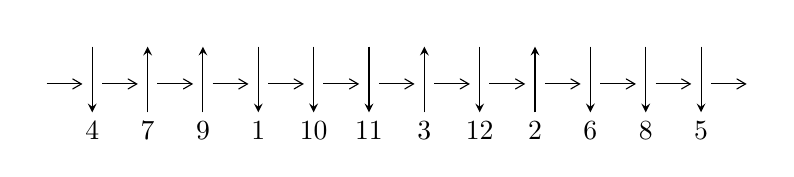
\begin{tikzpicture}[x=20pt, y=17pt]
	% nodes
	\node (C0) at (0, 0) {};
	\node (C1) at (1, 0) {};
	\node (C1U) at (1, +1) {};
	\node (C1D) at (1, -1) {4};

	\node (C2) at (2, 0) {};
	\node (C2U) at (2, +1) {};
	\node (C2D) at (2, -1) {7};

	\node (C3) at (3, 0) {};
	\node (C3U) at (3, +1) {};
	\node (C3D) at (3, -1) {9};

	\node (C4) at (4, 0) {};
	\node (C4U) at (4, +1) {};
	\node (C4D) at (4, -1) {1};

	\node (C5) at (5, 0) {};
	\node (C5U) at (5, +1) {};
	\node (C5D) at (5, -1) {10};

	\node (C6) at (6, 0) {};
	\node (C6U) at (6, +1) {};
	\node (C6D) at (6, -1) {11};

	\node (C7) at (7, 0) {};
	\node (C7U) at (7, +1) {};
	\node (C7D) at (7, -1) {3};

	\node (C8) at (8, 0) {};
	\node (C8U) at (8, +1) {};
	\node (C8D) at (8, -1) {12};

	\node (C9) at (9, 0) {};
	\node (C9U) at (9, +1) {};
	\node (C9D) at (9, -1) {2};

	\node (C10) at (10, 0) {};
	\node (C10U) at (10, +1) {};
	\node (C10D) at (10, -1) {6};

	\node (C11) at (11, 0) {};
	\node (C11U) at (11, +1) {};
	\node (C11D) at (11, -1) {8};

	\node (C12) at (12, 0) {};
	\node (C12U) at (12, +1) {};
	\node (C12D) at (12, -1) {5};
	\node (C13) at (13, 0) {};

	% arrows
	\draw[->,>={angle 60}]
	(C0) edge (C1) (C1) edge (C2) (C2) edge (C3) (C3) edge (C4) (C4) edge (C5) (C5) edge (C6) (C6) edge (C7) (C7) edge (C8) (C8) edge (C9) (C9) edge (C10) (C10) edge (C11) (C11) edge (C12) (C12) edge (C13) ;	\draw[->,>=stealth]
	(C1U) edge (C1D) (C2D) edge (C2U) (C3D) edge (C3U) (C4U) edge (C4D) (C5U) edge (C5D) (C6U) edge (C6D) (C7D) edge (C7U) (C8U) edge (C8D) (C9D) edge (C9U) (C10U) edge (C10D) (C11U) edge (C11D) (C12U) edge (C12D) ;
	\end{tikzpicture} \\
\hhline{~~} \\& 
\textbf{Solving Sequence} \\ \cline{2-2} 
 &
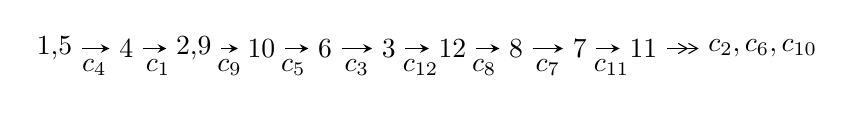
\begin{tikzpicture}[x=23pt, y=7pt]
	% node
	\node (A0) at (-1/8, 0) {1,5};
	\node (A1) at (1, 0) {4};
	\node (A2) at (33/16, 0) {2,9};
	\node (A3) at (25/8, 0) {10};
	\node (A4) at (33/8, 0) {6};
	\node (A5) at (41/8, 0) {3};
	\node (A6) at (49/8, 0) {12};
	\node (A7) at (57/8, 0) {8};
	\node (A8) at (65/8, 0) {7};
	\node (A9) at (73/8, 0) {11};
	\node (C1) at (1/2, -1) {$c_{4}$};
	\node (C2) at (3/2, -1) {$c_{1}$};
	\node (C3) at (21/8, -1) {$c_{9}$};
	\node (C4) at (29/8, -1) {$c_{5}$};
	\node (C5) at (37/8, -1) {$c_{3}$};
	\node (C6) at (45/8, -1) {$c_{12}$};
	\node (C7) at (53/8, -1) {$c_{8}$};
	\node (C8) at (61/8, -1) {$c_{7}$};
	\node (C9) at (69/8, -1) {$c_{11}$};
	\node (A10) at (11, 0) {$c_{2},c_{6},c_{10}$};

	% edge
	\draw[->,>=stealth]	
	(A0) edge (A1) (A1) edge (A2) (A2) edge (A3) (A3) edge (A4) (A4) edge (A5) (A5) edge (A6) (A6) edge (A7) (A7) edge (A8) (A8) edge (A9) ;
	\draw[->>,>={angle 60}]	
	(A9) edge (A10);
\end{tikzpicture} \\ 

\end{tabular} \\

\footnotetext{
The image of knot diagram is generated by the software ``\textbf{Draw programme}" developed by Andrew Bartholomew(\url{http://www.layer8.co.uk/maths/draw/index.htm\#Running-draw}), where we modified some parts for our purpose(\url{https://github.com/CATsTAILs/LinksPainter}).
}\phantom \\ \newline 
\centering \textbf{Ideals for irreducible components\footnotemark of $X_{\text{par}}$} 
 
\begin{align*}
I^u_{1}&=\langle 
-6.17416\times10^{167} u^{107}+1.20918\times10^{168} u^{106}+\cdots+4.51045\times10^{167} b+1.01541\times10^{170},\\
\phantom{I^u_{1}}&\phantom{= \langle  }-1.07213\times10^{170} u^{107}+1.67093\times10^{170} u^{106}+\cdots+7.06637\times10^{168} a+1.11521\times10^{172},\\
\phantom{I^u_{1}}&\phantom{= \langle  }u^{108}-2 u^{107}+\cdots-299 u+47\rangle \\
I^u_{2}&=\langle 
- u^{26}-3 u^{25}+\cdots+b-1,\;-4 u^{26}-10 u^{25}+\cdots+a+5,\;u^{27}+3 u^{26}+\cdots+6 u+1\rangle \\
\\
\end{align*}
\raggedright * 2 irreducible components of $\dim_{\mathbb{C}}=0$, with total 135 representations.\\
\footnotetext{All coefficients of polynomials are rational numbers. But the coefficients are sometimes approximated in decimal forms when there is not enough margin.}
\newpage
\renewcommand{\arraystretch}{1}
\centering \section*{I. $I^u_{1}= \langle -6.17\times10^{167} u^{107}+1.21\times10^{168} u^{106}+\cdots+4.51\times10^{167} b+1.02\times10^{170},\;-1.07\times10^{170} u^{107}+1.67\times10^{170} u^{106}+\cdots+7.07\times10^{168} a+1.12\times10^{172},\;u^{108}-2 u^{107}+\cdots-299 u+47 \rangle$}
\flushleft \textbf{(i) Arc colorings}\\
\begin{tabular}{m{7pt} m{180pt} m{7pt} m{180pt} }
\flushright $a_{1}=$&$\begin{pmatrix}0\\u\end{pmatrix}$ \\
\flushright $a_{5}=$&$\begin{pmatrix}1\\0\end{pmatrix}$ \\
\flushright $a_{4}=$&$\begin{pmatrix}1\\- u^2\end{pmatrix}$ \\
\flushright $a_{2}=$&$\begin{pmatrix}- u\\u^3+u\end{pmatrix}$ \\
\flushright $a_{9}=$&$\begin{pmatrix}15.1723 u^{107}-23.6463 u^{106}+\cdots+6660.78 u-1578.19\\1.36886 u^{107}-2.68085 u^{106}+\cdots+921.712 u-225.124\end{pmatrix}$ \\
\flushright $a_{10}=$&$\begin{pmatrix}20.0873 u^{107}-30.6623 u^{106}+\cdots+8396.19 u-2000.20\\-3.49659 u^{107}+5.45677 u^{106}+\cdots-1424.06 u+329.133\end{pmatrix}$ \\
\flushright $a_{6}=$&$\begin{pmatrix}28.1414 u^{107}-43.5083 u^{106}+\cdots+11918.4 u-2851.74\\-8.48372 u^{107}+13.3771 u^{106}+\cdots-3599.41 u+861.349\end{pmatrix}$ \\
\flushright $a_{3}=$&$\begin{pmatrix}6.47264 u^{107}-9.65167 u^{106}+\cdots+2937.00 u-738.000\\5.66238 u^{107}-8.30970 u^{106}+\cdots+2515.37 u-615.722\end{pmatrix}$ \\
\flushright $a_{12}=$&$\begin{pmatrix}u\\u\end{pmatrix}$ \\
\flushright $a_{8}=$&$\begin{pmatrix}12.6300 u^{107}-19.1931 u^{106}+\cdots+5323.74 u-1266.05\\-1.17347 u^{107}+1.77231 u^{106}+\cdots-415.326 u+87.0247\end{pmatrix}$ \\
\flushright $a_{7}=$&$\begin{pmatrix}-0.134410 u^{107}+1.57897 u^{106}+\cdots-199.017 u+71.6823\\-8.59288 u^{107}+13.8267 u^{106}+\cdots-3500.53 u+823.438\end{pmatrix}$ \\
\flushright $a_{11}=$&$\begin{pmatrix}-17.2692 u^{107}+25.8300 u^{106}+\cdots-7157.94 u+1718.79\\11.0079 u^{107}-17.3057 u^{106}+\cdots+4803.68 u-1152.57\end{pmatrix}$\\&\end{tabular}
\flushleft \textbf{(ii) Obstruction class $= -1$}\\~\\
\flushleft \textbf{(iii) Cusp Shapes $= 133.129 u^{107}-204.954 u^{106}+\cdots+56643.2 u-13565.8$}\\~\\
\newpage\renewcommand{\arraystretch}{1}
\flushleft \textbf{(iv) u-Polynomials at the component}\newline \\
\begin{tabular}{m{50pt}|m{274pt}}
Crossings & \hspace{64pt}u-Polynomials at each crossing \\
\hline $$\begin{aligned}c_{1},c_{4},c_{12}\end{aligned}$$&$\begin{aligned}
&u^{108}-2 u^{107}+\cdots-299 u+47
\end{aligned}$\\
\hline $$\begin{aligned}c_{2},c_{7}\end{aligned}$$&$\begin{aligned}
&u^{108}+u^{107}+\cdots+u+1
\end{aligned}$\\
\hline $$\begin{aligned}c_{3}\end{aligned}$$&$\begin{aligned}
&u^{108}- u^{107}+\cdots-28281 u+2677
\end{aligned}$\\
\hline $$\begin{aligned}c_{5},c_{6},c_{10}\end{aligned}$$&$\begin{aligned}
&u^{108}- u^{107}+\cdots+575 u-103
\end{aligned}$\\
\hline $$\begin{aligned}c_{8},c_{11}\end{aligned}$$&$\begin{aligned}
&u^{108}-38 u^{106}+\cdots-2046 u+89
\end{aligned}$\\
\hline $$\begin{aligned}c_{9}\end{aligned}$$&$\begin{aligned}
&u^{108}+3 u^{107}+\cdots-492579 u+108211
\end{aligned}$\\
\hline
\end{tabular}\\~\\
\newpage\renewcommand{\arraystretch}{1}
\flushleft \textbf{(v) Riley Polynomials at the component}\newline \\
\begin{tabular}{m{50pt}|m{274pt}}
Crossings & \hspace{64pt}Riley Polynomials at each crossing \\
\hline $$\begin{aligned}c_{1},c_{4},c_{12}\end{aligned}$$&$\begin{aligned}
&y^{108}+102 y^{107}+\cdots-95417 y+2209
\end{aligned}$\\
\hline $$\begin{aligned}c_{2},c_{7}\end{aligned}$$&$\begin{aligned}
&y^{108}-55 y^{107}+\cdots-31 y+1
\end{aligned}$\\
\hline $$\begin{aligned}c_{3}\end{aligned}$$&$\begin{aligned}
&y^{108}-17 y^{107}+\cdots-304371863 y+7166329
\end{aligned}$\\
\hline $$\begin{aligned}c_{5},c_{6},c_{10}\end{aligned}$$&$\begin{aligned}
&y^{108}-109 y^{107}+\cdots-159233 y+10609
\end{aligned}$\\
\hline $$\begin{aligned}c_{8},c_{11}\end{aligned}$$&$\begin{aligned}
&y^{108}-76 y^{107}+\cdots-3384048 y+7921
\end{aligned}$\\
\hline $$\begin{aligned}c_{9}\end{aligned}$$&$\begin{aligned}
&y^{108}-13 y^{107}+\cdots+118667308219 y+11709620521
\end{aligned}$\\
\hline
\end{tabular}\\~\\
\newpage\flushleft \textbf{(vi) Complex Volumes and Cusp Shapes}
$$\begin{array}{c|c|c}  
\text{Solutions to }I^u_{1}& \I (\text{vol} + \sqrt{-1}CS) & \text{Cusp shape}\\
 \hline 
\begin{aligned}
u &= -0.960885 + 0.291199 I \\
a &= -0.249799 + 0.319511 I \\
b &= \phantom{-}1.048870 + 0.325112 I\end{aligned}
 & -9.01540 + 5.66019 I & \phantom{-0.000000 } 0 \\ \hline\begin{aligned}
u &= -0.960885 - 0.291199 I \\
a &= -0.249799 - 0.319511 I \\
b &= \phantom{-}1.048870 - 0.325112 I\end{aligned}
 & -9.01540 - 5.66019 I & \phantom{-0.000000 } 0 \\ \hline\begin{aligned}
u &= \phantom{-}0.879867 + 0.356835 I \\
a &= \phantom{-}0.463996 + 0.497326 I \\
b &= -1.100970 + 0.398607 I\end{aligned}
 & -6.4421 - 12.9182 I & \phantom{-0.000000 } 0 \\ \hline\begin{aligned}
u &= \phantom{-}0.879867 - 0.356835 I \\
a &= \phantom{-}0.463996 - 0.497326 I \\
b &= -1.100970 - 0.398607 I\end{aligned}
 & -6.4421 + 12.9182 I & \phantom{-0.000000 } 0 \\ \hline\begin{aligned}
u &= \phantom{-}0.915261\phantom{ +0.000000I} \\
a &= -0.232583\phantom{ +0.000000I} \\
b &= -1.24242\phantom{ +0.000000I}\end{aligned}
 & -0.201236\phantom{ +0.000000I} & \phantom{-0.000000 } 0 \\ \hline\begin{aligned}
u &= -0.756019 + 0.477784 I \\
a &= \phantom{-}0.290448 - 0.199196 I \\
b &= \phantom{-}0.079001 - 0.498921 I\end{aligned}
 & -4.52075 + 2.63427 I & \phantom{-0.000000 } 0 \\ \hline\begin{aligned}
u &= -0.756019 - 0.477784 I \\
a &= \phantom{-}0.290448 + 0.199196 I \\
b &= \phantom{-}0.079001 + 0.498921 I\end{aligned}
 & -4.52075 - 2.63427 I & \phantom{-0.000000 } 0 \\ \hline\begin{aligned}
u &= \phantom{-}0.607423 + 0.651574 I \\
a &= -0.371400 + 0.981234 I \\
b &= \phantom{-}0.129075 - 0.255913 I\end{aligned}
 & \phantom{-}0.66299 + 4.02428 I & \phantom{-0.000000 } 0 \\ \hline\begin{aligned}
u &= \phantom{-}0.607423 - 0.651574 I \\
a &= -0.371400 - 0.981234 I \\
b &= \phantom{-}0.129075 + 0.255913 I\end{aligned}
 & \phantom{-}0.66299 - 4.02428 I & \phantom{-0.000000 } 0 \\ \hline\begin{aligned}
u &= -0.629163 + 0.913726 I \\
a &= \phantom{-}0.046330 + 0.624056 I \\
b &= -0.360205 - 0.065003 I\end{aligned}
 & -1.34592 + 1.86587 I & \phantom{-0.000000 } 0\\
 \hline 
 \end{array}$$\newpage$$\begin{array}{c|c|c}  
\text{Solutions to }I^u_{1}& \I (\text{vol} + \sqrt{-1}CS) & \text{Cusp shape}\\
 \hline 
\begin{aligned}
u &= -0.629163 - 0.913726 I \\
a &= \phantom{-}0.046330 - 0.624056 I \\
b &= -0.360205 + 0.065003 I\end{aligned}
 & -1.34592 - 1.86587 I & \phantom{-0.000000 } 0 \\ \hline\begin{aligned}
u &= -0.799233 + 0.384923 I \\
a &= \phantom{-}0.393026 - 0.191895 I \\
b &= -0.780162 - 0.402902 I\end{aligned}
 & -2.75619 + 3.19878 I & \phantom{-0.000000 } 0 \\ \hline\begin{aligned}
u &= -0.799233 - 0.384923 I \\
a &= \phantom{-}0.393026 + 0.191895 I \\
b &= -0.780162 + 0.402902 I\end{aligned}
 & -2.75619 - 3.19878 I & \phantom{-0.000000 } 0 \\ \hline\begin{aligned}
u &= \phantom{-}0.680217 + 0.881835 I \\
a &= \phantom{-}0.110805 - 0.836202 I \\
b &= -0.113620 + 0.333723 I\end{aligned}
 & -4.89449 + 7.56548 I & \phantom{-0.000000 } 0 \\ \hline\begin{aligned}
u &= \phantom{-}0.680217 - 0.881835 I \\
a &= \phantom{-}0.110805 + 0.836202 I \\
b &= -0.113620 - 0.333723 I\end{aligned}
 & -4.89449 - 7.56548 I & \phantom{-0.000000 } 0 \\ \hline\begin{aligned}
u &= -0.713702 + 0.467724 I \\
a &= \phantom{-}0.685472 - 0.609005 I \\
b &= -0.214722 - 0.196909 I\end{aligned}
 & -4.55568 + 2.15661 I & \phantom{-0.000000 } 0 \\ \hline\begin{aligned}
u &= -0.713702 - 0.467724 I \\
a &= \phantom{-}0.685472 + 0.609005 I \\
b &= -0.214722 + 0.196909 I\end{aligned}
 & -4.55568 - 2.15661 I & \phantom{-0.000000 } 0 \\ \hline\begin{aligned}
u &= \phantom{-}0.741551 + 0.400490 I \\
a &= -0.532830 - 0.358069 I \\
b &= \phantom{-}1.077380 - 0.535396 I\end{aligned}
 & -0.12708 - 8.61802 I & \phantom{-0.000000 } 0 \\ \hline\begin{aligned}
u &= \phantom{-}0.741551 - 0.400490 I \\
a &= -0.532830 + 0.358069 I \\
b &= \phantom{-}1.077380 + 0.535396 I\end{aligned}
 & -0.12708 + 8.61802 I & \phantom{-0.000000 } 0 \\ \hline\begin{aligned}
u &= -0.871367 + 0.785491 I \\
a &= -0.015895 - 0.166669 I \\
b &= \phantom{-}0.471406 - 0.061492 I\end{aligned}
 & -4.51827 + 3.11099 I & \phantom{-0.000000 } 0\\
 \hline 
 \end{array}$$\newpage$$\begin{array}{c|c|c}  
\text{Solutions to }I^u_{1}& \I (\text{vol} + \sqrt{-1}CS) & \text{Cusp shape}\\
 \hline 
\begin{aligned}
u &= -0.871367 - 0.785491 I \\
a &= -0.015895 + 0.166669 I \\
b &= \phantom{-}0.471406 + 0.061492 I\end{aligned}
 & -4.51827 - 3.11099 I & \phantom{-0.000000 } 0 \\ \hline\begin{aligned}
u &= \phantom{-}0.628602 + 0.514592 I \\
a &= \phantom{-}0.140119 + 0.038698 I \\
b &= -0.942555 - 0.441495 I\end{aligned}
 & -2.52085 + 2.11298 I & \phantom{-0.000000 } 0 \\ \hline\begin{aligned}
u &= \phantom{-}0.628602 - 0.514592 I \\
a &= \phantom{-}0.140119 - 0.038698 I \\
b &= -0.942555 + 0.441495 I\end{aligned}
 & -2.52085 - 2.11298 I & \phantom{-0.000000 } 0 \\ \hline\begin{aligned}
u &= \phantom{-}0.658355 + 0.427540 I \\
a &= -0.50852 - 1.37677 I \\
b &= \phantom{-}0.167600 + 0.058679 I\end{aligned}
 & -2.76561 - 6.36964 I & \phantom{-0.000000 } 0 \\ \hline\begin{aligned}
u &= \phantom{-}0.658355 - 0.427540 I \\
a &= -0.50852 + 1.37677 I \\
b &= \phantom{-}0.167600 - 0.058679 I\end{aligned}
 & -2.76561 + 6.36964 I & \phantom{-0.000000 } 0 \\ \hline\begin{aligned}
u &= -0.015750 + 1.241230 I \\
a &= -0.55862 - 1.97146 I \\
b &= -0.452918 - 0.930203 I\end{aligned}
 & \phantom{-}1.21460 + 1.83268 I & \phantom{-0.000000 } 0 \\ \hline\begin{aligned}
u &= -0.015750 - 1.241230 I \\
a &= -0.55862 + 1.97146 I \\
b &= -0.452918 + 0.930203 I\end{aligned}
 & \phantom{-}1.21460 - 1.83268 I & \phantom{-0.000000 } 0 \\ \hline\begin{aligned}
u &= -0.000500 + 1.271320 I \\
a &= -0.490111 - 0.034234 I \\
b &= -0.735300 + 1.164510 I\end{aligned}
 & \phantom{-}1.49298 - 1.58324 I & \phantom{-0.000000 } 0 \\ \hline\begin{aligned}
u &= -0.000500 - 1.271320 I \\
a &= -0.490111 + 0.034234 I \\
b &= -0.735300 - 1.164510 I\end{aligned}
 & \phantom{-}1.49298 + 1.58324 I & \phantom{-0.000000 } 0 \\ \hline\begin{aligned}
u &= -0.139816 + 1.267230 I \\
a &= -2.81942 - 0.52924 I \\
b &= -2.80141 - 1.17487 I\end{aligned}
 & -3.26505 - 2.41999 I & \phantom{-0.000000 } 0\\
 \hline 
 \end{array}$$\newpage$$\begin{array}{c|c|c}  
\text{Solutions to }I^u_{1}& \I (\text{vol} + \sqrt{-1}CS) & \text{Cusp shape}\\
 \hline 
\begin{aligned}
u &= -0.139816 - 1.267230 I \\
a &= -2.81942 + 0.52924 I \\
b &= -2.80141 + 1.17487 I\end{aligned}
 & -3.26505 + 2.41999 I & \phantom{-0.000000 } 0 \\ \hline\begin{aligned}
u &= -0.668451 + 1.095630 I \\
a &= \phantom{-}0.175348 - 0.759921 I \\
b &= \phantom{-}0.397156 + 0.121065 I\end{aligned}
 & -6.66351 + 0.05480 I & \phantom{-0.000000 } 0 \\ \hline\begin{aligned}
u &= -0.668451 - 1.095630 I \\
a &= \phantom{-}0.175348 + 0.759921 I \\
b &= \phantom{-}0.397156 - 0.121065 I\end{aligned}
 & -6.66351 - 0.05480 I & \phantom{-0.000000 } 0 \\ \hline\begin{aligned}
u &= -0.114982 + 1.283170 I \\
a &= -2.17584 - 0.88097 I \\
b &= -3.09042 - 1.67081 I\end{aligned}
 & -2.89688 + 5.98499 I & \phantom{-0.000000 } 0 \\ \hline\begin{aligned}
u &= -0.114982 - 1.283170 I \\
a &= -2.17584 + 0.88097 I \\
b &= -3.09042 + 1.67081 I\end{aligned}
 & -2.89688 - 5.98499 I & \phantom{-0.000000 } 0 \\ \hline\begin{aligned}
u &= \phantom{-}0.145553 + 1.285280 I \\
a &= \phantom{-}2.14352 - 0.14424 I \\
b &= \phantom{-}2.38908 - 1.20652 I\end{aligned}
 & -5.82754 - 2.11330 I & \phantom{-0.000000 } 0 \\ \hline\begin{aligned}
u &= \phantom{-}0.145553 - 1.285280 I \\
a &= \phantom{-}2.14352 + 0.14424 I \\
b &= \phantom{-}2.38908 + 1.20652 I\end{aligned}
 & -5.82754 + 2.11330 I & \phantom{-0.000000 } 0 \\ \hline\begin{aligned}
u &= \phantom{-}0.139891 + 1.303940 I \\
a &= \phantom{-}1.46519 - 0.44271 I \\
b &= \phantom{-}1.84127 - 1.77249 I\end{aligned}
 & -5.64315 - 2.18598 I & \phantom{-0.000000 } 0 \\ \hline\begin{aligned}
u &= \phantom{-}0.139891 - 1.303940 I \\
a &= \phantom{-}1.46519 + 0.44271 I \\
b &= \phantom{-}1.84127 + 1.77249 I\end{aligned}
 & -5.64315 + 2.18598 I & \phantom{-0.000000 } 0 \\ \hline\begin{aligned}
u &= \phantom{-}0.165819 + 1.311960 I \\
a &= \phantom{-}0.827554 + 0.648288 I \\
b &= \phantom{-}0.961060 - 0.559226 I\end{aligned}
 & -5.48555 - 2.56883 I & \phantom{-0.000000 } 0\\
 \hline 
 \end{array}$$\newpage$$\begin{array}{c|c|c}  
\text{Solutions to }I^u_{1}& \I (\text{vol} + \sqrt{-1}CS) & \text{Cusp shape}\\
 \hline 
\begin{aligned}
u &= \phantom{-}0.165819 - 1.311960 I \\
a &= \phantom{-}0.827554 - 0.648288 I \\
b &= \phantom{-}0.961060 + 0.559226 I\end{aligned}
 & -5.48555 + 2.56883 I & \phantom{-0.000000 } 0 \\ \hline\begin{aligned}
u &= -0.184266 + 1.314620 I \\
a &= -0.45129 + 1.65609 I \\
b &= -0.726779 + 0.686118 I\end{aligned}
 & -2.60615 + 7.32685 I & \phantom{-0.000000 } 0 \\ \hline\begin{aligned}
u &= -0.184266 - 1.314620 I \\
a &= -0.45129 - 1.65609 I \\
b &= -0.726779 - 0.686118 I\end{aligned}
 & -2.60615 - 7.32685 I & \phantom{-0.000000 } 0 \\ \hline\begin{aligned}
u &= \phantom{-}0.520457 + 0.421420 I \\
a &= \phantom{-}0.333578 + 1.304730 I \\
b &= -0.406578 + 0.125920 I\end{aligned}
 & \phantom{-}3.42972 - 3.43786 I & \phantom{-0.000000 -}0. + 7.18170 I \\ \hline\begin{aligned}
u &= \phantom{-}0.520457 - 0.421420 I \\
a &= \phantom{-}0.333578 - 1.304730 I \\
b &= -0.406578 - 0.125920 I\end{aligned}
 & \phantom{-}3.42972 + 3.43786 I & \phantom{-0.000000 } 0. - 7.18170 I \\ \hline\begin{aligned}
u &= -0.163049 + 1.336820 I \\
a &= \phantom{-}0.379416 + 0.145811 I \\
b &= \phantom{-}0.674270 - 1.070430 I\end{aligned}
 & -2.12910 - 1.69175 I & \phantom{-0.000000 } 0 \\ \hline\begin{aligned}
u &= -0.163049 - 1.336820 I \\
a &= \phantom{-}0.379416 - 0.145811 I \\
b &= \phantom{-}0.674270 + 1.070430 I\end{aligned}
 & -2.12910 + 1.69175 I & \phantom{-0.000000 } 0 \\ \hline\begin{aligned}
u &= \phantom{-}0.009254 + 1.382140 I \\
a &= -1.375880 + 0.064550 I \\
b &= -1.80279 + 0.63837 I\end{aligned}
 & \phantom{-}3.07345 - 0.98640 I & \phantom{-0.000000 } 0 \\ \hline\begin{aligned}
u &= \phantom{-}0.009254 - 1.382140 I \\
a &= -1.375880 - 0.064550 I \\
b &= -1.80279 - 0.63837 I\end{aligned}
 & \phantom{-}3.07345 + 0.98640 I & \phantom{-0.000000 } 0 \\ \hline\begin{aligned}
u &= \phantom{-}0.112915 + 1.384630 I \\
a &= \phantom{-}2.07144 + 0.39362 I \\
b &= \phantom{-}2.45982 + 0.63773 I\end{aligned}
 & \phantom{-}8.06931 - 1.78241 I & \phantom{-0.000000 } 0\\
 \hline 
 \end{array}$$\newpage$$\begin{array}{c|c|c}  
\text{Solutions to }I^u_{1}& \I (\text{vol} + \sqrt{-1}CS) & \text{Cusp shape}\\
 \hline 
\begin{aligned}
u &= \phantom{-}0.112915 - 1.384630 I \\
a &= \phantom{-}2.07144 - 0.39362 I \\
b &= \phantom{-}2.45982 - 0.63773 I\end{aligned}
 & \phantom{-}8.06931 + 1.78241 I & \phantom{-0.000000 } 0 \\ \hline\begin{aligned}
u &= \phantom{-}0.513028 + 0.316851 I \\
a &= \phantom{-}0.791650 + 0.093355 I \\
b &= -1.25958 + 0.75068 I\end{aligned}
 & -0.92372 - 3.05623 I & -6.12777 + 7.79662 I \\ \hline\begin{aligned}
u &= \phantom{-}0.513028 - 0.316851 I \\
a &= \phantom{-}0.791650 - 0.093355 I \\
b &= -1.25958 - 0.75068 I\end{aligned}
 & -0.92372 + 3.05623 I & -6.12777 - 7.79662 I \\ \hline\begin{aligned}
u &= \phantom{-}0.556846 + 0.210177 I \\
a &= \phantom{-}1.38483 - 0.74285 I \\
b &= -0.254810 + 0.168021 I\end{aligned}
 & -1.199540 + 0.252286 I & -7.51222 + 1.35320 I \\ \hline\begin{aligned}
u &= \phantom{-}0.556846 - 0.210177 I \\
a &= \phantom{-}1.38483 + 0.74285 I \\
b &= -0.254810 - 0.168021 I\end{aligned}
 & -1.199540 - 0.252286 I & -7.51222 - 1.35320 I \\ \hline\begin{aligned}
u &= \phantom{-}0.526995 + 0.270176 I \\
a &= \phantom{-}0.196728 - 0.611934 I \\
b &= \phantom{-}0.898486 + 0.021517 I\end{aligned}
 & \phantom{-}3.10533 + 0.11149 I & \phantom{-}1.82107 + 0.90182 I \\ \hline\begin{aligned}
u &= \phantom{-}0.526995 - 0.270176 I \\
a &= \phantom{-}0.196728 + 0.611934 I \\
b &= \phantom{-}0.898486 - 0.021517 I\end{aligned}
 & \phantom{-}3.10533 - 0.11149 I & \phantom{-}1.82107 - 0.90182 I \\ \hline\begin{aligned}
u &= \phantom{-}0.409524 + 1.347340 I \\
a &= -1.31749 - 0.89229 I \\
b &= -1.61711 - 0.28044 I\end{aligned}
 & \phantom{-}4.06832 - 4.76863 I & \phantom{-0.000000 } 0 \\ \hline\begin{aligned}
u &= \phantom{-}0.409524 - 1.347340 I \\
a &= -1.31749 + 0.89229 I \\
b &= -1.61711 + 0.28044 I\end{aligned}
 & \phantom{-}4.06832 + 4.76863 I & \phantom{-0.000000 } 0 \\ \hline\begin{aligned}
u &= -0.18631 + 1.40377 I \\
a &= \phantom{-}2.01754 + 0.72985 I \\
b &= \phantom{-}2.19802 + 1.28966 I\end{aligned}
 & \phantom{-}3.95477 + 2.14843 I & \phantom{-0.000000 } 0\\
 \hline 
 \end{array}$$\newpage$$\begin{array}{c|c|c}  
\text{Solutions to }I^u_{1}& \I (\text{vol} + \sqrt{-1}CS) & \text{Cusp shape}\\
 \hline 
\begin{aligned}
u &= -0.18631 - 1.40377 I \\
a &= \phantom{-}2.01754 - 0.72985 I \\
b &= \phantom{-}2.19802 - 1.28966 I\end{aligned}
 & \phantom{-}3.95477 - 2.14843 I & \phantom{-0.000000 } 0 \\ \hline\begin{aligned}
u &= -0.15134 + 1.41016 I \\
a &= \phantom{-}1.53834 + 0.42907 I \\
b &= \phantom{-}2.28622 + 1.00208 I\end{aligned}
 & \phantom{-}4.08170 + 4.86816 I & \phantom{-0.000000 } 0 \\ \hline\begin{aligned}
u &= -0.15134 - 1.41016 I \\
a &= \phantom{-}1.53834 - 0.42907 I \\
b &= \phantom{-}2.28622 - 1.00208 I\end{aligned}
 & \phantom{-}4.08170 - 4.86816 I & \phantom{-0.000000 } 0 \\ \hline\begin{aligned}
u &= \phantom{-}0.26018 + 1.40612 I \\
a &= \phantom{-}0.312189 + 0.489836 I \\
b &= \phantom{-}0.422413 + 1.152420 I\end{aligned}
 & \phantom{-}3.95143 - 2.93911 I & \phantom{-0.000000 } 0 \\ \hline\begin{aligned}
u &= \phantom{-}0.26018 - 1.40612 I \\
a &= \phantom{-}0.312189 - 0.489836 I \\
b &= \phantom{-}0.422413 - 1.152420 I\end{aligned}
 & \phantom{-}3.95143 + 2.93911 I & \phantom{-0.000000 } 0 \\ \hline\begin{aligned}
u &= \phantom{-}0.27858 + 1.40857 I \\
a &= \phantom{-}1.50777 + 0.66400 I \\
b &= \phantom{-}2.00793 + 0.23819 I\end{aligned}
 & \phantom{-}8.27314 - 3.13426 I & \phantom{-0.000000 } 0 \\ \hline\begin{aligned}
u &= \phantom{-}0.27858 - 1.40857 I \\
a &= \phantom{-}1.50777 - 0.66400 I \\
b &= \phantom{-}2.00793 - 0.23819 I\end{aligned}
 & \phantom{-}8.27314 + 3.13426 I & \phantom{-0.000000 } 0 \\ \hline\begin{aligned}
u &= \phantom{-}0.20327 + 1.42244 I \\
a &= -2.42805 + 0.22092 I \\
b &= -2.84613 + 1.06570 I\end{aligned}
 & \phantom{-}4.66794 - 5.74198 I & \phantom{-0.000000 } 0 \\ \hline\begin{aligned}
u &= \phantom{-}0.20327 - 1.42244 I \\
a &= -2.42805 - 0.22092 I \\
b &= -2.84613 - 1.06570 I\end{aligned}
 & \phantom{-}4.66794 + 5.74198 I & \phantom{-0.000000 } 0 \\ \hline\begin{aligned}
u &= -0.14687 + 1.43811 I \\
a &= \phantom{-}1.169270 + 0.044649 I \\
b &= \phantom{-}1.60540 - 0.16218 I\end{aligned}
 & \phantom{-}5.57039 + 2.71636 I & \phantom{-0.000000 } 0\\
 \hline 
 \end{array}$$\newpage$$\begin{array}{c|c|c}  
\text{Solutions to }I^u_{1}& \I (\text{vol} + \sqrt{-1}CS) & \text{Cusp shape}\\
 \hline 
\begin{aligned}
u &= -0.14687 - 1.43811 I \\
a &= \phantom{-}1.169270 - 0.044649 I \\
b &= \phantom{-}1.60540 + 0.16218 I\end{aligned}
 & \phantom{-}5.57039 - 2.71636 I & \phantom{-0.000000 } 0 \\ \hline\begin{aligned}
u &= -0.492215 + 0.249012 I \\
a &= -0.824121 + 0.198501 I \\
b &= \phantom{-}0.688523 + 1.133750 I\end{aligned}
 & -1.356930 - 0.364886 I & -7.63760 - 1.14677 I \\ \hline\begin{aligned}
u &= -0.492215 - 0.249012 I \\
a &= -0.824121 - 0.198501 I \\
b &= \phantom{-}0.688523 - 1.133750 I\end{aligned}
 & -1.356930 + 0.364886 I & -7.63760 + 1.14677 I \\ \hline\begin{aligned}
u &= \phantom{-}0.18750 + 1.45044 I \\
a &= -1.63241 - 0.36166 I \\
b &= -2.40745 - 0.61245 I\end{aligned}
 & \phantom{-}9.45327 - 6.03947 I & \phantom{-0.000000 } 0 \\ \hline\begin{aligned}
u &= \phantom{-}0.18750 - 1.45044 I \\
a &= -1.63241 + 0.36166 I \\
b &= -2.40745 + 0.61245 I\end{aligned}
 & \phantom{-}9.45327 + 6.03947 I & \phantom{-0.000000 } 0 \\ \hline\begin{aligned}
u &= -0.523236 + 0.062547 I \\
a &= \phantom{-}0.837529 + 0.934705 I \\
b &= -1.33607 + 1.11209 I\end{aligned}
 & -6.94722 + 4.75131 I & -11.69397 - 4.35447 I \\ \hline\begin{aligned}
u &= -0.523236 - 0.062547 I \\
a &= \phantom{-}0.837529 - 0.934705 I \\
b &= -1.33607 - 1.11209 I\end{aligned}
 & -6.94722 - 4.75131 I & -11.69397 + 4.35447 I \\ \hline\begin{aligned}
u &= \phantom{-}0.24247 + 1.46432 I \\
a &= \phantom{-}1.42620 + 0.45731 I \\
b &= \phantom{-}2.42437 + 0.79189 I\end{aligned}
 & \phantom{-}3.32012 - 9.65966 I & \phantom{-0.000000 } 0 \\ \hline\begin{aligned}
u &= \phantom{-}0.24247 - 1.46432 I \\
a &= \phantom{-}1.42620 - 0.45731 I \\
b &= \phantom{-}2.42437 - 0.79189 I\end{aligned}
 & \phantom{-}3.32012 + 9.65966 I & \phantom{-0.000000 } 0 \\ \hline\begin{aligned}
u &= -0.444548 + 0.248062 I \\
a &= -2.07093 + 0.35714 I \\
b &= \phantom{-}0.334505 + 0.408255 I\end{aligned}
 & -1.23188 + 2.67764 I & -8.00090 - 10.68725 I\\
 \hline 
 \end{array}$$\newpage$$\begin{array}{c|c|c}  
\text{Solutions to }I^u_{1}& \I (\text{vol} + \sqrt{-1}CS) & \text{Cusp shape}\\
 \hline 
\begin{aligned}
u &= -0.444548 - 0.248062 I \\
a &= -2.07093 - 0.35714 I \\
b &= \phantom{-}0.334505 - 0.408255 I\end{aligned}
 & -1.23188 - 2.67764 I & -8.00090 + 10.68725 I \\ \hline\begin{aligned}
u &= -0.28802 + 1.46360 I \\
a &= -1.63445 - 0.11403 I \\
b &= -2.09049 - 0.75480 I\end{aligned}
 & \phantom{-}3.18901 + 7.09486 I & \phantom{-0.000000 } 0 \\ \hline\begin{aligned}
u &= -0.28802 - 1.46360 I \\
a &= -1.63445 + 0.11403 I \\
b &= -2.09049 + 0.75480 I\end{aligned}
 & \phantom{-}3.18901 - 7.09486 I & \phantom{-0.000000 } 0 \\ \hline\begin{aligned}
u &= \phantom{-}0.27537 + 1.46680 I \\
a &= \phantom{-}2.08401 - 0.14935 I \\
b &= \phantom{-}2.65186 - 0.94698 I\end{aligned}
 & \phantom{-}5.88295 - 12.31150 I & \phantom{-0.000000 } 0 \\ \hline\begin{aligned}
u &= \phantom{-}0.27537 - 1.46680 I \\
a &= \phantom{-}2.08401 + 0.14935 I \\
b &= \phantom{-}2.65186 + 0.94698 I\end{aligned}
 & \phantom{-}5.88295 + 12.31150 I & \phantom{-0.000000 } 0 \\ \hline\begin{aligned}
u &= -0.28845 + 1.46832 I \\
a &= -0.844057 - 0.322078 I \\
b &= -1.006910 - 0.429078 I\end{aligned}
 & \phantom{-}1.66920 + 6.47731 I & \phantom{-0.000000 } 0 \\ \hline\begin{aligned}
u &= -0.28845 - 1.46832 I \\
a &= -0.844057 + 0.322078 I \\
b &= -1.006910 + 0.429078 I\end{aligned}
 & \phantom{-}1.66920 - 6.47731 I & \phantom{-0.000000 } 0 \\ \hline\begin{aligned}
u &= \phantom{-}0.18394 + 1.48641 I \\
a &= -1.45002 - 0.36108 I \\
b &= -2.13938 + 0.17582 I\end{aligned}
 & \phantom{-}4.06961 - 0.77391 I & \phantom{-0.000000 } 0 \\ \hline\begin{aligned}
u &= \phantom{-}0.18394 - 1.48641 I \\
a &= -1.45002 + 0.36108 I \\
b &= -2.13938 - 0.17582 I\end{aligned}
 & \phantom{-}4.06961 + 0.77391 I & \phantom{-0.000000 } 0 \\ \hline\begin{aligned}
u &= \phantom{-}0.498781 + 0.031813 I \\
a &= -1.83780 + 0.78218 I \\
b &= \phantom{-}1.200940 + 0.443882 I\end{aligned}
 & -9.72324 - 0.17260 I & -14.6955 - 1.6811 I\\
 \hline 
 \end{array}$$\newpage$$\begin{array}{c|c|c}  
\text{Solutions to }I^u_{1}& \I (\text{vol} + \sqrt{-1}CS) & \text{Cusp shape}\\
 \hline 
\begin{aligned}
u &= \phantom{-}0.498781 - 0.031813 I \\
a &= -1.83780 - 0.78218 I \\
b &= \phantom{-}1.200940 - 0.443882 I\end{aligned}
 & -9.72324 + 0.17260 I & -14.6955 + 1.6811 I \\ \hline\begin{aligned}
u &= -0.26046 + 1.47949 I \\
a &= -1.350680 - 0.064524 I \\
b &= -2.13964 - 0.22084 I\end{aligned}
 & \phantom{-}1.70234 + 5.70571 I & \phantom{-0.000000 } 0 \\ \hline\begin{aligned}
u &= -0.26046 - 1.47949 I \\
a &= -1.350680 + 0.064524 I \\
b &= -2.13964 + 0.22084 I\end{aligned}
 & \phantom{-}1.70234 - 5.70571 I & \phantom{-0.000000 } 0 \\ \hline\begin{aligned}
u &= -0.37688 + 1.45966 I \\
a &= \phantom{-}1.65237 - 0.15351 I \\
b &= \phantom{-}2.15867 + 0.62908 I\end{aligned}
 & -3.41289 + 10.44450 I & \phantom{-0.000000 } 0 \\ \hline\begin{aligned}
u &= -0.37688 - 1.45966 I \\
a &= \phantom{-}1.65237 + 0.15351 I \\
b &= \phantom{-}2.15867 - 0.62908 I\end{aligned}
 & -3.41289 - 10.44450 I & \phantom{-0.000000 } 0 \\ \hline\begin{aligned}
u &= \phantom{-}0.13345 + 1.50197 I \\
a &= -0.651574 - 0.494247 I \\
b &= -1.00228 - 1.08760 I\end{aligned}
 & \phantom{-}7.84173 + 1.60885 I & \phantom{-0.000000 } 0 \\ \hline\begin{aligned}
u &= \phantom{-}0.13345 - 1.50197 I \\
a &= -0.651574 + 0.494247 I \\
b &= -1.00228 + 1.08760 I\end{aligned}
 & \phantom{-}7.84173 - 1.60885 I & \phantom{-0.000000 } 0 \\ \hline\begin{aligned}
u &= \phantom{-}0.34024 + 1.47130 I \\
a &= -1.95397 - 0.02823 I \\
b &= -2.63237 + 0.78593 I\end{aligned}
 & -0.5823 - 17.3216 I & \phantom{-0.000000 } 0 \\ \hline\begin{aligned}
u &= \phantom{-}0.34024 - 1.47130 I \\
a &= -1.95397 + 0.02823 I \\
b &= -2.63237 - 0.78593 I\end{aligned}
 & -0.5823 + 17.3216 I & \phantom{-0.000000 } 0 \\ \hline\begin{aligned}
u &= \phantom{-}0.474941\phantom{ +0.000000I} \\
a &= -2.72071\phantom{ +0.000000I} \\
b &= \phantom{-}0.983847\phantom{ +0.000000I}\end{aligned}
 & -9.72586\phantom{ +0.000000I} & -24.9570\phantom{ +0.000000I}\\
 \hline 
 \end{array}$$\newpage$$\begin{array}{c|c|c}  
\text{Solutions to }I^u_{1}& \I (\text{vol} + \sqrt{-1}CS) & \text{Cusp shape}\\
 \hline 
\begin{aligned}
u &= -0.465572 + 0.075078 I \\
a &= \phantom{-}1.94842 + 2.59870 I \\
b &= -0.579859 + 0.622820 I\end{aligned}
 & -6.63078 - 3.98358 I & -12.51677 + 2.81229 I \\ \hline\begin{aligned}
u &= -0.465572 - 0.075078 I \\
a &= \phantom{-}1.94842 - 2.59870 I \\
b &= -0.579859 - 0.622820 I\end{aligned}
 & -6.63078 + 3.98358 I & -12.51677 - 2.81229 I \\ \hline\begin{aligned}
u &= -0.326714 + 0.306052 I \\
a &= -0.490568 + 0.740050 I \\
b &= \phantom{-}0.055279 + 0.356898 I\end{aligned}
 & -0.167562 + 0.876730 I & -3.96855 - 7.53814 I \\ \hline\begin{aligned}
u &= -0.326714 - 0.306052 I \\
a &= -0.490568 - 0.740050 I \\
b &= \phantom{-}0.055279 - 0.356898 I\end{aligned}
 & -0.167562 - 0.876730 I & -3.96855 + 7.53814 I \\ \hline\begin{aligned}
u &= \phantom{-}0.441030\phantom{ +0.000000I} \\
a &= \phantom{-}1.00462\phantom{ +0.000000I} \\
b &= \phantom{-}1.11644\phantom{ +0.000000I}\end{aligned}
 & \phantom{-}3.20630\phantom{ +0.000000I} & \phantom{-}6.32680\phantom{ +0.000000I} \\ \hline\begin{aligned}
u &= -0.01728 + 1.56600 I \\
a &= \phantom{-}0.999723 + 0.344621 I \\
b &= \phantom{-}1.54938 + 0.87919 I\end{aligned}
 & \phantom{-}4.21990 + 5.75104 I & \phantom{-0.000000 } 0 \\ \hline\begin{aligned}
u &= -0.01728 - 1.56600 I \\
a &= \phantom{-}0.999723 - 0.344621 I \\
b &= \phantom{-}1.54938 - 0.87919 I\end{aligned}
 & \phantom{-}4.21990 - 5.75104 I & \phantom{-0.000000 } 0 \\ \hline\begin{aligned}
u &= \phantom{-}0.338766\phantom{ +0.000000I} \\
a &= \phantom{-}1.91535\phantom{ +0.000000I} \\
b &= -0.532834\phantom{ +0.000000I}\end{aligned}
 & -1.44061\phantom{ +0.000000I} & -6.16230\phantom{ +0.000000I}\\
 \hline 
 \end{array}$$\newpage\newpage\renewcommand{\arraystretch}{1}
\centering \section*{II. $I^u_{2}= \langle - u^{26}-3 u^{25}+\cdots+b-1,\;-4 u^{26}-10 u^{25}+\cdots+a+5,\;u^{27}+3 u^{26}+\cdots+6 u+1 \rangle$}
\flushleft \textbf{(i) Arc colorings}\\
\begin{tabular}{m{7pt} m{180pt} m{7pt} m{180pt} }
\flushright $a_{1}=$&$\begin{pmatrix}0\\u\end{pmatrix}$ \\
\flushright $a_{5}=$&$\begin{pmatrix}1\\0\end{pmatrix}$ \\
\flushright $a_{4}=$&$\begin{pmatrix}1\\- u^2\end{pmatrix}$ \\
\flushright $a_{2}=$&$\begin{pmatrix}- u\\u^3+u\end{pmatrix}$ \\
\flushright $a_{9}=$&$\begin{pmatrix}4 u^{26}+10 u^{25}+\cdots-19 u-5\\u^{26}+3 u^{25}+\cdots+7 u+1\end{pmatrix}$ \\
\flushright $a_{10}=$&$\begin{pmatrix}7 u^{26}+17 u^{25}+\cdots-19 u-5\\4 u^{26}+10 u^{25}+\cdots-2 u-1\end{pmatrix}$ \\
\flushright $a_{6}=$&$\begin{pmatrix}-2 u^{26}-6 u^{25}+\cdots-39 u-7\\2 u^{26}+12 u^{25}+\cdots+24 u+4\end{pmatrix}$ \\
\flushright $a_{3}=$&$\begin{pmatrix}-3 u^{26}-12 u^{25}+\cdots-40 u-6\\-3 u^{25}-7 u^{24}+\cdots+4 u^2+3 u\end{pmatrix}$ \\
\flushright $a_{12}=$&$\begin{pmatrix}u\\u\end{pmatrix}$ \\
\flushright $a_{8}=$&$\begin{pmatrix}10 u^{26}+26 u^{25}+\cdots-28 u-7\\7 u^{26}+19 u^{25}+\cdots-2 u-1\end{pmatrix}$ \\
\flushright $a_{7}=$&$\begin{pmatrix}4 u^{26}+16 u^{25}+\cdots+22 u^2-3 u\\2 u^{26}+6 u^{25}+\cdots+9 u^2+4 u\end{pmatrix}$ \\
\flushright $a_{11}=$&$\begin{pmatrix}-4 u^{26}-12 u^{25}+\cdots-18 u-6\\-3 u^{26}-7 u^{25}+\cdots+13 u+4\end{pmatrix}$\\&\end{tabular}
\flushleft \textbf{(ii) Obstruction class $= 1$}\\~\\
\flushleft \textbf{(iii) Cusp Shapes $= 8 u^{26}+14 u^{25}+108 u^{24}+159 u^{23}+627 u^{22}+764 u^{21}+2034 u^{20}+1955 u^{19}+3971 u^{18}+2638 u^{17}+4608 u^{16}+1110 u^{15}+2804 u^{14}-1918 u^{13}+482 u^{12}-3380 u^{11}-123 u^{10}-2436 u^9+250 u^8-1025 u^7+301 u^6-248 u^5+147 u^4-6 u^3+29 u^2- u-5$}\\~\\
\newpage\renewcommand{\arraystretch}{1}
\flushleft \textbf{(iv) u-Polynomials at the component}\newline \\
\begin{tabular}{m{50pt}|m{274pt}}
Crossings & \hspace{64pt}u-Polynomials at each crossing \\
\hline $$\begin{aligned}c_{1},c_{12}\end{aligned}$$&$\begin{aligned}
&u^{27}-3 u^{26}+\cdots+6 u-1
\end{aligned}$\\
\hline $$\begin{aligned}c_{2}\end{aligned}$$&$\begin{aligned}
&u^{27}-9 u^{25}+\cdots-9 u^2+1
\end{aligned}$\\
\hline $$\begin{aligned}c_{3}\end{aligned}$$&$\begin{aligned}
&u^{27}-2 u^{24}+\cdots-9 u^2-1
\end{aligned}$\\
\hline $$\begin{aligned}c_{4}\end{aligned}$$&$\begin{aligned}
&u^{27}+3 u^{26}+\cdots+6 u+1
\end{aligned}$\\
\hline $$\begin{aligned}c_{5},c_{6}\end{aligned}$$&$\begin{aligned}
&u^{27}-16 u^{25}+\cdots-6 u+1
\end{aligned}$\\
\hline $$\begin{aligned}c_{7}\end{aligned}$$&$\begin{aligned}
&u^{27}-9 u^{25}+\cdots+9 u^2-1
\end{aligned}$\\
\hline $$\begin{aligned}c_{8}\end{aligned}$$&$\begin{aligned}
&u^{27}+5 u^{26}+\cdots-5 u-1
\end{aligned}$\\
\hline $$\begin{aligned}c_{9}\end{aligned}$$&$\begin{aligned}
&u^{27}+7 u^{24}+\cdots+6 u-1
\end{aligned}$\\
\hline $$\begin{aligned}c_{10}\end{aligned}$$&$\begin{aligned}
&u^{27}-16 u^{25}+\cdots-6 u-1
\end{aligned}$\\
\hline $$\begin{aligned}c_{11}\end{aligned}$$&$\begin{aligned}
&u^{27}-5 u^{26}+\cdots-5 u+1
\end{aligned}$\\
\hline
\end{tabular}\\~\\
\newpage\renewcommand{\arraystretch}{1}
\flushleft \textbf{(v) Riley Polynomials at the component}\newline \\
\begin{tabular}{m{50pt}|m{274pt}}
Crossings & \hspace{64pt}Riley Polynomials at each crossing \\
\hline $$\begin{aligned}c_{1},c_{4},c_{12}\end{aligned}$$&$\begin{aligned}
&y^{27}+27 y^{26}+\cdots-8 y-1
\end{aligned}$\\
\hline $$\begin{aligned}c_{2},c_{7}\end{aligned}$$&$\begin{aligned}
&y^{27}-18 y^{26}+\cdots+18 y-1
\end{aligned}$\\
\hline $$\begin{aligned}c_{3}\end{aligned}$$&$\begin{aligned}
&y^{27}-14 y^{25}+\cdots-18 y-1
\end{aligned}$\\
\hline $$\begin{aligned}c_{5},c_{6},c_{10}\end{aligned}$$&$\begin{aligned}
&y^{27}-32 y^{26}+\cdots+16 y-1
\end{aligned}$\\
\hline $$\begin{aligned}c_{8},c_{11}\end{aligned}$$&$\begin{aligned}
&y^{27}-27 y^{26}+\cdots+23 y-1
\end{aligned}$\\
\hline $$\begin{aligned}c_{9}\end{aligned}$$&$\begin{aligned}
&y^{27}+4 y^{25}+\cdots-32 y-1
\end{aligned}$\\
\hline
\end{tabular}\\~\\
\newpage\flushleft \textbf{(vi) Complex Volumes and Cusp Shapes}
$$\begin{array}{c|c|c}  
\text{Solutions to }I^u_{2}& \I (\text{vol} + \sqrt{-1}CS) & \text{Cusp shape}\\
 \hline 
\begin{aligned}
u &= -0.349187 + 0.950871 I \\
a &= -0.807587 + 0.771242 I \\
b &= -1.121300 - 0.478024 I\end{aligned}
 & -7.80198 + 1.43571 I & -9.19532 - 2.58353 I \\ \hline\begin{aligned}
u &= -0.349187 - 0.950871 I \\
a &= -0.807587 - 0.771242 I \\
b &= -1.121300 + 0.478024 I\end{aligned}
 & -7.80198 - 1.43571 I & -9.19532 + 2.58353 I \\ \hline\begin{aligned}
u &= -0.524782 + 0.805011 I \\
a &= -0.191943 - 0.585590 I \\
b &= \phantom{-}0.429680 + 0.206238 I\end{aligned}
 & -1.56889 + 2.18949 I & -7.93685 - 8.86415 I \\ \hline\begin{aligned}
u &= -0.524782 - 0.805011 I \\
a &= -0.191943 + 0.585590 I \\
b &= \phantom{-}0.429680 - 0.206238 I\end{aligned}
 & -1.56889 - 2.18949 I & -7.93685 + 8.86415 I \\ \hline\begin{aligned}
u &= \phantom{-}0.865146\phantom{ +0.000000I} \\
a &= \phantom{-}0.399939\phantom{ +0.000000I} \\
b &= \phantom{-}0.830267\phantom{ +0.000000I}\end{aligned}
 & \phantom{-}0.961761\phantom{ +0.000000I} & -1.58940\phantom{ +0.000000I} \\ \hline\begin{aligned}
u &= -0.894303 + 0.699265 I \\
a &= \phantom{-}0.343752 + 0.029060 I \\
b &= -0.168841 - 0.129023 I\end{aligned}
 & -4.88580 + 3.15924 I & -20.5341 - 9.3982 I \\ \hline\begin{aligned}
u &= -0.894303 - 0.699265 I \\
a &= \phantom{-}0.343752 - 0.029060 I \\
b &= -0.168841 + 0.129023 I\end{aligned}
 & -4.88580 - 3.15924 I & -20.5341 + 9.3982 I \\ \hline\begin{aligned}
u &= \phantom{-}0.029596 + 1.250160 I \\
a &= \phantom{-}2.13970 + 0.39451 I \\
b &= \phantom{-}2.65297 - 0.60411 I\end{aligned}
 & -2.85769 - 4.49481 I & -3.90049 + 2.81559 I \\ \hline\begin{aligned}
u &= \phantom{-}0.029596 - 1.250160 I \\
a &= \phantom{-}2.13970 - 0.39451 I \\
b &= \phantom{-}2.65297 + 0.60411 I\end{aligned}
 & -2.85769 + 4.49481 I & -3.90049 - 2.81559 I \\ \hline\begin{aligned}
u &= -0.032871 + 1.304030 I \\
a &= -0.160820 - 0.814359 I \\
b &= -0.329944 + 0.286174 I\end{aligned}
 & \phantom{-}2.29000 - 1.19742 I & \phantom{-}2.58030 - 0.47093 I\\
 \hline 
 \end{array}$$\newpage$$\begin{array}{c|c|c}  
\text{Solutions to }I^u_{2}& \I (\text{vol} + \sqrt{-1}CS) & \text{Cusp shape}\\
 \hline 
\begin{aligned}
u &= -0.032871 - 1.304030 I \\
a &= -0.160820 + 0.814359 I \\
b &= -0.329944 - 0.286174 I\end{aligned}
 & \phantom{-}2.29000 + 1.19742 I & \phantom{-}2.58030 + 0.47093 I \\ \hline\begin{aligned}
u &= -0.122293 + 1.328560 I \\
a &= -1.64806 - 0.35102 I \\
b &= -1.96596 - 1.71147 I\end{aligned}
 & -5.28712 + 1.88129 I & \phantom{-}3.03676 + 4.91413 I \\ \hline\begin{aligned}
u &= -0.122293 - 1.328560 I \\
a &= -1.64806 + 0.35102 I \\
b &= -1.96596 + 1.71147 I\end{aligned}
 & -5.28712 - 1.88129 I & \phantom{-}3.03676 - 4.91413 I \\ \hline\begin{aligned}
u &= \phantom{-}0.207564 + 1.370530 I \\
a &= -1.96759 - 0.60435 I \\
b &= -2.31426 - 0.20194 I\end{aligned}
 & \phantom{-}7.35928 - 2.72940 I & -3.54297 + 2.72914 I \\ \hline\begin{aligned}
u &= \phantom{-}0.207564 - 1.370530 I \\
a &= -1.96759 + 0.60435 I \\
b &= -2.31426 + 0.20194 I\end{aligned}
 & \phantom{-}7.35928 + 2.72940 I & -3.54297 - 2.72914 I \\ \hline\begin{aligned}
u &= \phantom{-}0.35746 + 1.38079 I \\
a &= \phantom{-}1.120110 + 0.669009 I \\
b &= \phantom{-}1.45233 + 0.47462 I\end{aligned}
 & \phantom{-}5.42748 - 4.43200 I & \phantom{-}0.67537 + 3.40706 I \\ \hline\begin{aligned}
u &= \phantom{-}0.35746 - 1.38079 I \\
a &= \phantom{-}1.120110 - 0.669009 I \\
b &= \phantom{-}1.45233 - 0.47462 I\end{aligned}
 & \phantom{-}5.42748 + 4.43200 I & \phantom{-}0.67537 - 3.40706 I \\ \hline\begin{aligned}
u &= -0.027004 + 0.563292 I \\
a &= \phantom{-}1.91164 + 1.44067 I \\
b &= \phantom{-}0.941661 - 0.329293 I\end{aligned}
 & -5.44454 + 4.33420 I & -5.60921 - 3.77384 I \\ \hline\begin{aligned}
u &= -0.027004 - 0.563292 I \\
a &= \phantom{-}1.91164 - 1.44067 I \\
b &= \phantom{-}0.941661 + 0.329293 I\end{aligned}
 & -5.44454 - 4.33420 I & -5.60921 + 3.77384 I \\ \hline\begin{aligned}
u &= -0.15542 + 1.44244 I \\
a &= \phantom{-}1.73021 + 0.57101 I \\
b &= \phantom{-}2.28253 + 1.18196 I\end{aligned}
 & \phantom{-}4.64936 + 3.70031 I & \phantom{-}0.96546 - 2.09491 I\\
 \hline 
 \end{array}$$\newpage$$\begin{array}{c|c|c}  
\text{Solutions to }I^u_{2}& \I (\text{vol} + \sqrt{-1}CS) & \text{Cusp shape}\\
 \hline 
\begin{aligned}
u &= -0.15542 - 1.44244 I \\
a &= \phantom{-}1.73021 - 0.57101 I \\
b &= \phantom{-}2.28253 - 1.18196 I\end{aligned}
 & \phantom{-}4.64936 - 3.70031 I & \phantom{-}0.96546 + 2.09491 I \\ \hline\begin{aligned}
u &= \phantom{-}0.542990\phantom{ +0.000000I} \\
a &= -0.340066\phantom{ +0.000000I} \\
b &= -1.35539\phantom{ +0.000000I}\end{aligned}
 & \phantom{-}2.82244\phantom{ +0.000000I} & -15.1650\phantom{ +0.000000I} \\ \hline\begin{aligned}
u &= -0.24899 + 1.51498 I \\
a &= -0.915730 - 0.316585 I \\
b &= -1.44310 - 0.51838 I\end{aligned}
 & \phantom{-}2.29278 + 6.93609 I & -0.88072 - 10.03541 I \\ \hline\begin{aligned}
u &= -0.24899 - 1.51498 I \\
a &= -0.915730 + 0.316585 I \\
b &= -1.44310 + 0.51838 I\end{aligned}
 & \phantom{-}2.29278 - 6.93609 I & -0.88072 + 10.03541 I \\ \hline\begin{aligned}
u &= -0.415767\phantom{ +0.000000I} \\
a &= \phantom{-}3.11726\phantom{ +0.000000I} \\
b &= -1.16114\phantom{ +0.000000I}\end{aligned}
 & -9.51393\phantom{ +0.000000I} & \phantom{-}13.4630\phantom{ +0.000000I} \\ \hline\begin{aligned}
u &= -0.235946 + 0.296409 I \\
a &= -2.14224 - 1.06325 I \\
b &= \phantom{-}0.427373 + 0.736804 I\end{aligned}
 & -1.17761 + 1.87746 I & -7.51263 - 1.01338 I \\ \hline\begin{aligned}
u &= -0.235946 - 0.296409 I \\
a &= -2.14224 + 1.06325 I \\
b &= \phantom{-}0.427373 - 0.736804 I\end{aligned}
 & -1.17761 - 1.87746 I & -7.51263 + 1.01338 I\\
 \hline 
 \end{array}$$\newpage
\newpage\renewcommand{\arraystretch}{1}
\centering \section*{ III. u-Polynomials}
\begin{tabular}{m{50pt}|m{274pt}}
Crossings & \hspace{64pt}u-Polynomials at each crossing \\
\hline $$\begin{aligned}c_{1},c_{12}\end{aligned}$$&$\begin{aligned}
&(u^{27}-3 u^{26}+\cdots+6 u-1)(u^{108}-2 u^{107}+\cdots-299 u+47)
\end{aligned}$\\
\hline $$\begin{aligned}c_{2}\end{aligned}$$&$\begin{aligned}
&(u^{27}-9 u^{25}+\cdots-9 u^2+1)(u^{108}+u^{107}+\cdots+u+1)
\end{aligned}$\\
\hline $$\begin{aligned}c_{3}\end{aligned}$$&$\begin{aligned}
&(u^{27}-2 u^{24}+\cdots-9 u^2-1)(u^{108}- u^{107}+\cdots-28281 u+2677)
\end{aligned}$\\
\hline $$\begin{aligned}c_{4}\end{aligned}$$&$\begin{aligned}
&(u^{27}+3 u^{26}+\cdots+6 u+1)(u^{108}-2 u^{107}+\cdots-299 u+47)
\end{aligned}$\\
\hline $$\begin{aligned}c_{5},c_{6}\end{aligned}$$&$\begin{aligned}
&(u^{27}-16 u^{25}+\cdots-6 u+1)(u^{108}- u^{107}+\cdots+575 u-103)
\end{aligned}$\\
\hline $$\begin{aligned}c_{7}\end{aligned}$$&$\begin{aligned}
&(u^{27}-9 u^{25}+\cdots+9 u^2-1)(u^{108}+u^{107}+\cdots+u+1)
\end{aligned}$\\
\hline $$\begin{aligned}c_{8}\end{aligned}$$&$\begin{aligned}
&(u^{27}+5 u^{26}+\cdots-5 u-1)(u^{108}-38 u^{106}+\cdots-2046 u+89)
\end{aligned}$\\
\hline $$\begin{aligned}c_{9}\end{aligned}$$&$\begin{aligned}
&(u^{27}+7 u^{24}+\cdots+6 u-1)(u^{108}+3 u^{107}+\cdots-492579 u+108211)
\end{aligned}$\\
\hline $$\begin{aligned}c_{10}\end{aligned}$$&$\begin{aligned}
&(u^{27}-16 u^{25}+\cdots-6 u-1)(u^{108}- u^{107}+\cdots+575 u-103)
\end{aligned}$\\
\hline $$\begin{aligned}c_{11}\end{aligned}$$&$\begin{aligned}
&(u^{27}-5 u^{26}+\cdots-5 u+1)(u^{108}-38 u^{106}+\cdots-2046 u+89)
\end{aligned}$\\
\hline
\end{tabular}\newpage\renewcommand{\arraystretch}{1}
\centering \section*{ IV. Riley Polynomials}
\begin{tabular}{m{50pt}|m{274pt}}
Crossings & \hspace{64pt}Riley Polynomials at each crossing \\
\hline $$\begin{aligned}c_{1},c_{4},c_{12}\end{aligned}$$&$\begin{aligned}
&(y^{27}+27 y^{26}+\cdots-8 y-1)(y^{108}+102 y^{107}+\cdots-95417 y+2209)
\end{aligned}$\\
\hline $$\begin{aligned}c_{2},c_{7}\end{aligned}$$&$\begin{aligned}
&(y^{27}-18 y^{26}+\cdots+18 y-1)(y^{108}-55 y^{107}+\cdots-31 y+1)
\end{aligned}$\\
\hline $$\begin{aligned}c_{3}\end{aligned}$$&$\begin{aligned}
&(y^{27}-14 y^{25}+\cdots-18 y-1)\\
&\cdot(y^{108}-17 y^{107}+\cdots-304371863 y+7166329)
\end{aligned}$\\
\hline $$\begin{aligned}c_{5},c_{6},c_{10}\end{aligned}$$&$\begin{aligned}
&(y^{27}-32 y^{26}+\cdots+16 y-1)\\
&\cdot(y^{108}-109 y^{107}+\cdots-159233 y+10609)
\end{aligned}$\\
\hline $$\begin{aligned}c_{8},c_{11}\end{aligned}$$&$\begin{aligned}
&(y^{27}-27 y^{26}+\cdots+23 y-1)(y^{108}-76 y^{107}+\cdots-3384048 y+7921)
\end{aligned}$\\
\hline $$\begin{aligned}c_{9}\end{aligned}$$&$\begin{aligned}
&(y^{27}+4 y^{25}+\cdots-32 y-1)\\
&\cdot(y^{108}-13 y^{107}+\cdots+118667308219 y+11709620521)
\end{aligned}$\\
\hline
\end{tabular}
\vskip 2pc
\end{document}